\documentclass[11pt]{article}
\usepackage[margin=0.9in]{geometry}
\usepackage{booktabs,graphicx,float,amsmath,xcolor,enumitem}
\usepackage[hidelinks]{hyperref}
\usepackage{titlesec}
\titleformat{\section}{\large\bfseries}{\thesection.}{0.5em}{}
\titleformat{\subsection}{\normalsize\bfseries}{}{0em}{}
\titlespacing*{\section}{0pt}{8pt}{3pt}
\titlespacing*{\subsection}{0pt}{8pt}{2pt}
\setlength{\parindent}{0pt}
\setlength{\parskip}{4pt}
\setlist{nosep,leftmargin=1.2em}
\setlist[itemize]{label=\textbullet}
\newcommand{\taurct}{\hat\tau^{\,\mathrm{RCT}}}

\begin{document}

\begin{center}
{\Large\bfseries Do City Chiefs Grant More Discretionary Tax Exemptions?}

\vspace{4pt}
\textbf{Name:} Tsu Ning Tsao \quad \textbf{Student Number:} 1012713137
\end{center}

\textbf{Research summary.} When neighbourhood chiefs (Local) instead of state agents (Central) collect the property tax, do more properties get exempted, and are the extra exemptions justified by the owner's legal status or discretionary favours? \textbf{Data:} replication data of Bal\'an et al.\ (2022), 2018 property-tax campaign in Kananga, D.R.\ Congo; neighbourhoods (\texttt{a7}) were randomly assigned to Central (\texttt{tmt}=1) or Local (\texttt{tmt}=2); the unit is the property. \textbf{Variables:} outcome $Y$ = \texttt{exempt} (1 if the collector registered the property as exempt); treatment $T$ = \texttt{local}; pre-treatment covariates $X$ = owner age, female, Luluwa (main tribe), works for the state.

\textbf{Track: RCT. Dataset used everywhere below: the full experimental sample} (5,645 properties in 202 neighbourhoods; 2,884 Local, 2,761 Central). The Week 6 biased sample is not used this week. Code: \texttt{Week8/00\_master/00\_master.py} $\rightarrow$ \texttt{02\_analysis/02\_week8\_metalearners.py}; outputs in \texttt{03\_output/week8/}.

\section{S-Learner, T-Learner and X-Learner (full experimental sample)}

\subsection{Step 1: Implementation and preferred learner}
\begin{itemize}
\item \textbf{Base learner.} All three learners use the same gradient-boosted regression tree (\texttt{GradientBoostingRegressor}, learning rate 0.05). I chose depth 3, 100 trees and at least 100 properties per leaf by 5-fold cross-validation on the S-learner outcome model, with folds formed by neighbourhood (CV MSE 0.154 vs 0.219 for a constant). Estimation uses \texttt{econml.metalearners}, seed 1465.
\item \textbf{S-learner:} one model $\hat\mu(x,t)$ with $T$ as a feature; CATE $=\hat\mu(x,1)-\hat\mu(x,0)$. \textbf{T-learner:} separate models for Local and Central; CATE = difference of their predictions. \textbf{X-learner:} imputes each property's effect with the other arm's model, fits a second model to these imputed effects in each arm, and combines the two with the propensity score. Since $T$ is randomised by neighbourhood, I use the known design propensity (share Local, 0.51) rather than an estimated score.
\item \textbf{ATE} = mean CATE over the 5,645 properties. \textbf{SE / CI:} 200 bootstrap draws resampling neighbourhoods (the unit of randomisation), refitting all learners each time.
\item \textbf{Preferred: X-learner.} In my data the true effect is small (about 3 points on a 29\% base) and $T$ is only one of five inputs, so the regularised S-learner rarely splits on $T$ and shrinks the CATE towards zero. The T-learner fits each arm on only about 2,800 properties, so its CATE is the difference of two noisy predictions. The X-learner uses both arms for each effect and smooths the imputed effects in a second step, so it is less noisy than T and less shrunk than S. Its usual advantage, unbalanced arms, is small here (51/49), which is why T and X end up close.
\end{itemize}

\subsection{Step 2: Results and comparison}
\begin{table}[H]\centering\small
\caption{ATE and CATE distribution, full experimental sample ($N=5{,}645$).}
\resizebox{\linewidth}{!}{\begin{tabular}{lcccccccc}
\toprule
 & \multicolumn{3}{c}{ATE (mean CATE)} & & \multicolumn{4}{c}{CATE distribution}\\
\cmidrule(lr){2-4}\cmidrule(lr){6-9}
Learner & $\hat\tau$ & SE$^b$ & 95\% CI$^b$ & $\hat\tau-\hat\tau^{RCT}$ & SD & P5 & P95 & Share $<0$\\
\midrule
Benchmark $\hat\tau^{RCT}$ (OLS, $Y$ on $T$ and $X$) & 0.031 & 0.026$^c$ & & & & & & \\
\addlinespace
S-learner & 0.022 & 0.022 & [-0.018, 0.070] & -0.009 & 0.026 & 0.000 & 0.083 & 0.05\\
T-learner & 0.029 & 0.025 & [-0.020, 0.078] & -0.002 & 0.068 & -0.059 & 0.141 & 0.29\\
X-learner & 0.029 & 0.025 & [-0.020, 0.079] & -0.002 & 0.052 & -0.041 & 0.131 & 0.24\\
\bottomrule
\end{tabular}
}
\par\smallskip\footnotesize $^c$ SE clustered by neighbourhood. $^b$ Bootstrap SE and 95\% percentile CI: 200 draws resampling neighbourhoods, all learners refit in each draw, seed 1465. P5/P95: 5th/95th percentile of the property-level CATE.
\end{table}
\begin{figure}[H]\centering
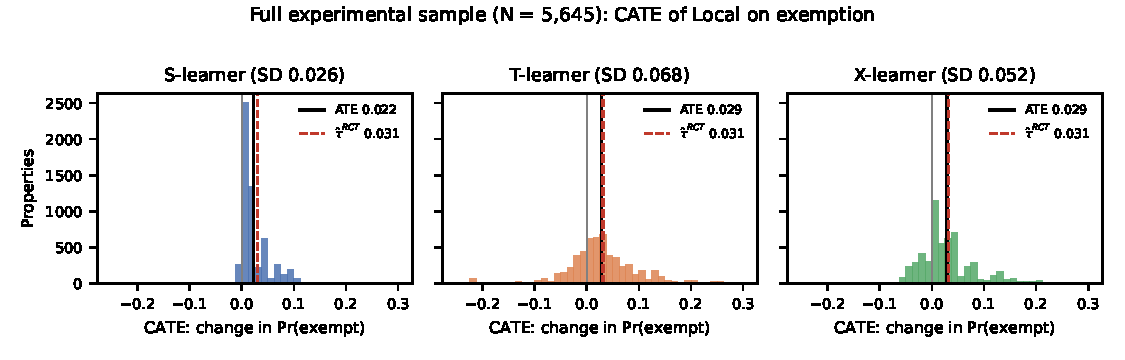
\includegraphics[width=\linewidth]{figure1_cate_hist.pdf}
\caption{Histogram of property-level CATEs, full experimental sample. Black line: ATE (mean CATE); red dashed line: $\taurct$.}
\end{figure}
\begin{itemize}
\item \textbf{All three ATEs are close to $\taurct=0.031$.} T and X give 0.029, a gap of 0.002. The S-learner gives 0.022, 0.009 below the benchmark but well inside one bootstrap SE (0.022). The gap is the regularisation bias described above: shrinking the effect of $T$ pulls the ATE towards zero. All CIs contain zero, as does the benchmark's. Local collection has no significant average effect on exemptions.
\item \textbf{The CATE distributions differ much more than the ATEs.} The S-learner is narrow (SD 0.026, 5\% negative). T is widest (SD 0.068, 29\% negative), and X is in between (SD 0.052). Since the bootstrap SE of the \emph{average} is already 0.025, much of the spread in T and X is likely estimation noise rather than real heterogeneity. These CATEs are also in-sample (fit and evaluated on the same properties), which adds spread.
\end{itemize}

\begin{figure}[H]\centering
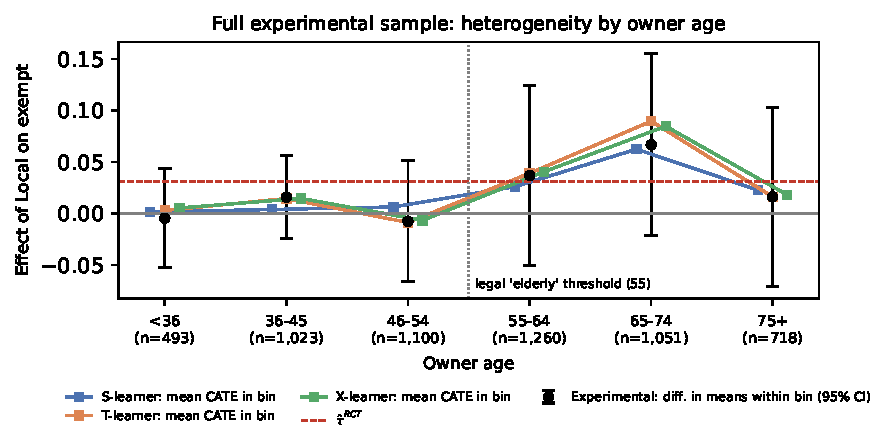
\includegraphics[width=0.78\linewidth]{figure2_cate_by_age.pdf}
\caption{Mean CATE by owner age bin vs the experimental difference in means within each bin, full experimental sample. Dotted line: 55, the legal age for an ``elderly'' exemption.}
\end{figure}
\begin{table}[H]\centering\small
\caption{Mean CATE by subgroup vs the experimental subgroup estimate, full experimental sample.}
\begin{tabular}{lrcccc}
\toprule
 & & Experimental & \multicolumn{3}{c}{Mean CATE in subgroup}\\
\cmidrule(lr){4-6}
Subgroup & $N$ & diff.\ in means (SE$^c$) & S & T & X\\
\midrule
Owner 55 or older & 3,029 & 0.034 (0.041) & 0.038 & 0.051 & 0.051\\
Owner under 55 & 2,616 & 0.002 (0.019) & 0.004 & 0.003 & 0.004\\
\addlinespace
Owner female & 1,482 & 0.034 (0.046) & 0.038 & 0.039 & 0.041\\
Owner male & 4,163 & 0.027 (0.029) & 0.017 & 0.025 & 0.024\\
\addlinespace
Owner Luluwa & 4,450 & 0.017 (0.033) & 0.023 & 0.032 & 0.031\\
Owner not Luluwa & 1,195 & 0.029 (0.049) & 0.019 & 0.015 & 0.022\\
\addlinespace
Owner works for state & 1,304 & 0.042 (0.039) & 0.023 & 0.041 & 0.043\\
Owner not state & 4,341 & 0.011 (0.033) & 0.022 & 0.025 & 0.025\\
\bottomrule
\end{tabular}

\par\smallskip\footnotesize Experimental: OLS of $Y$ on $T$ within the subgroup, SE clustered by neighbourhood.
\end{table}
\begin{itemize}
\item \textbf{The three learners agree on where the effect is.} It is essentially zero for owners under 55 (all learners 0.003--0.004; experiment 0.002). It sits among owners 55 and older (CATE 0.038--0.051; experiment 0.034) and peaks at ages 65--74. The learners follow the experimental by-bin estimates closely (Figure 2), which is a useful check that they are picking up signal and not noise.
\item \textbf{Link to the research question.} Under chiefs, the extra exemptions go to owners who are \emph{legally eligible} as elderly, not to younger owners. This points to justified rather than discretionary exemptions. It is only suggestive: the subgroup estimates are not significant (SE 0.041).
\item \textbf{Discrepancy.} T and X find a larger effect for owners who work for the state (0.041--0.043 vs 0.025), in line with the experiment (0.042 vs 0.011). The S-learner does not (0.023 vs 0.022): it only finds heterogeneity along owner age, the strongest predictor of the outcome itself. This is the same shrinkage problem, and another reason to prefer X.
\item \textbf{Next steps (Project 2).} Cross-fitted CATEs, a formal heterogeneity test (BLP / GATES) and the discretionary-exemption outcome.
\end{itemize}

\end{document}
